\chapter{Results}

\section{Requirements}

\section{Depth Camera}

\section{Heightmap}

\section{Walkability Scores}
    For testing the walkability scores described in section \ref{sec:scores}, a piece of terrain that demonstrates various types of obstacles
    that the robot might encounter was chosen, this terrain and its heightmap is shown in figure \ref{fig:score_test_map}.
    \begin{figure}[h]
        \centering
        \begin{subfigure}{.5\textwidth}
            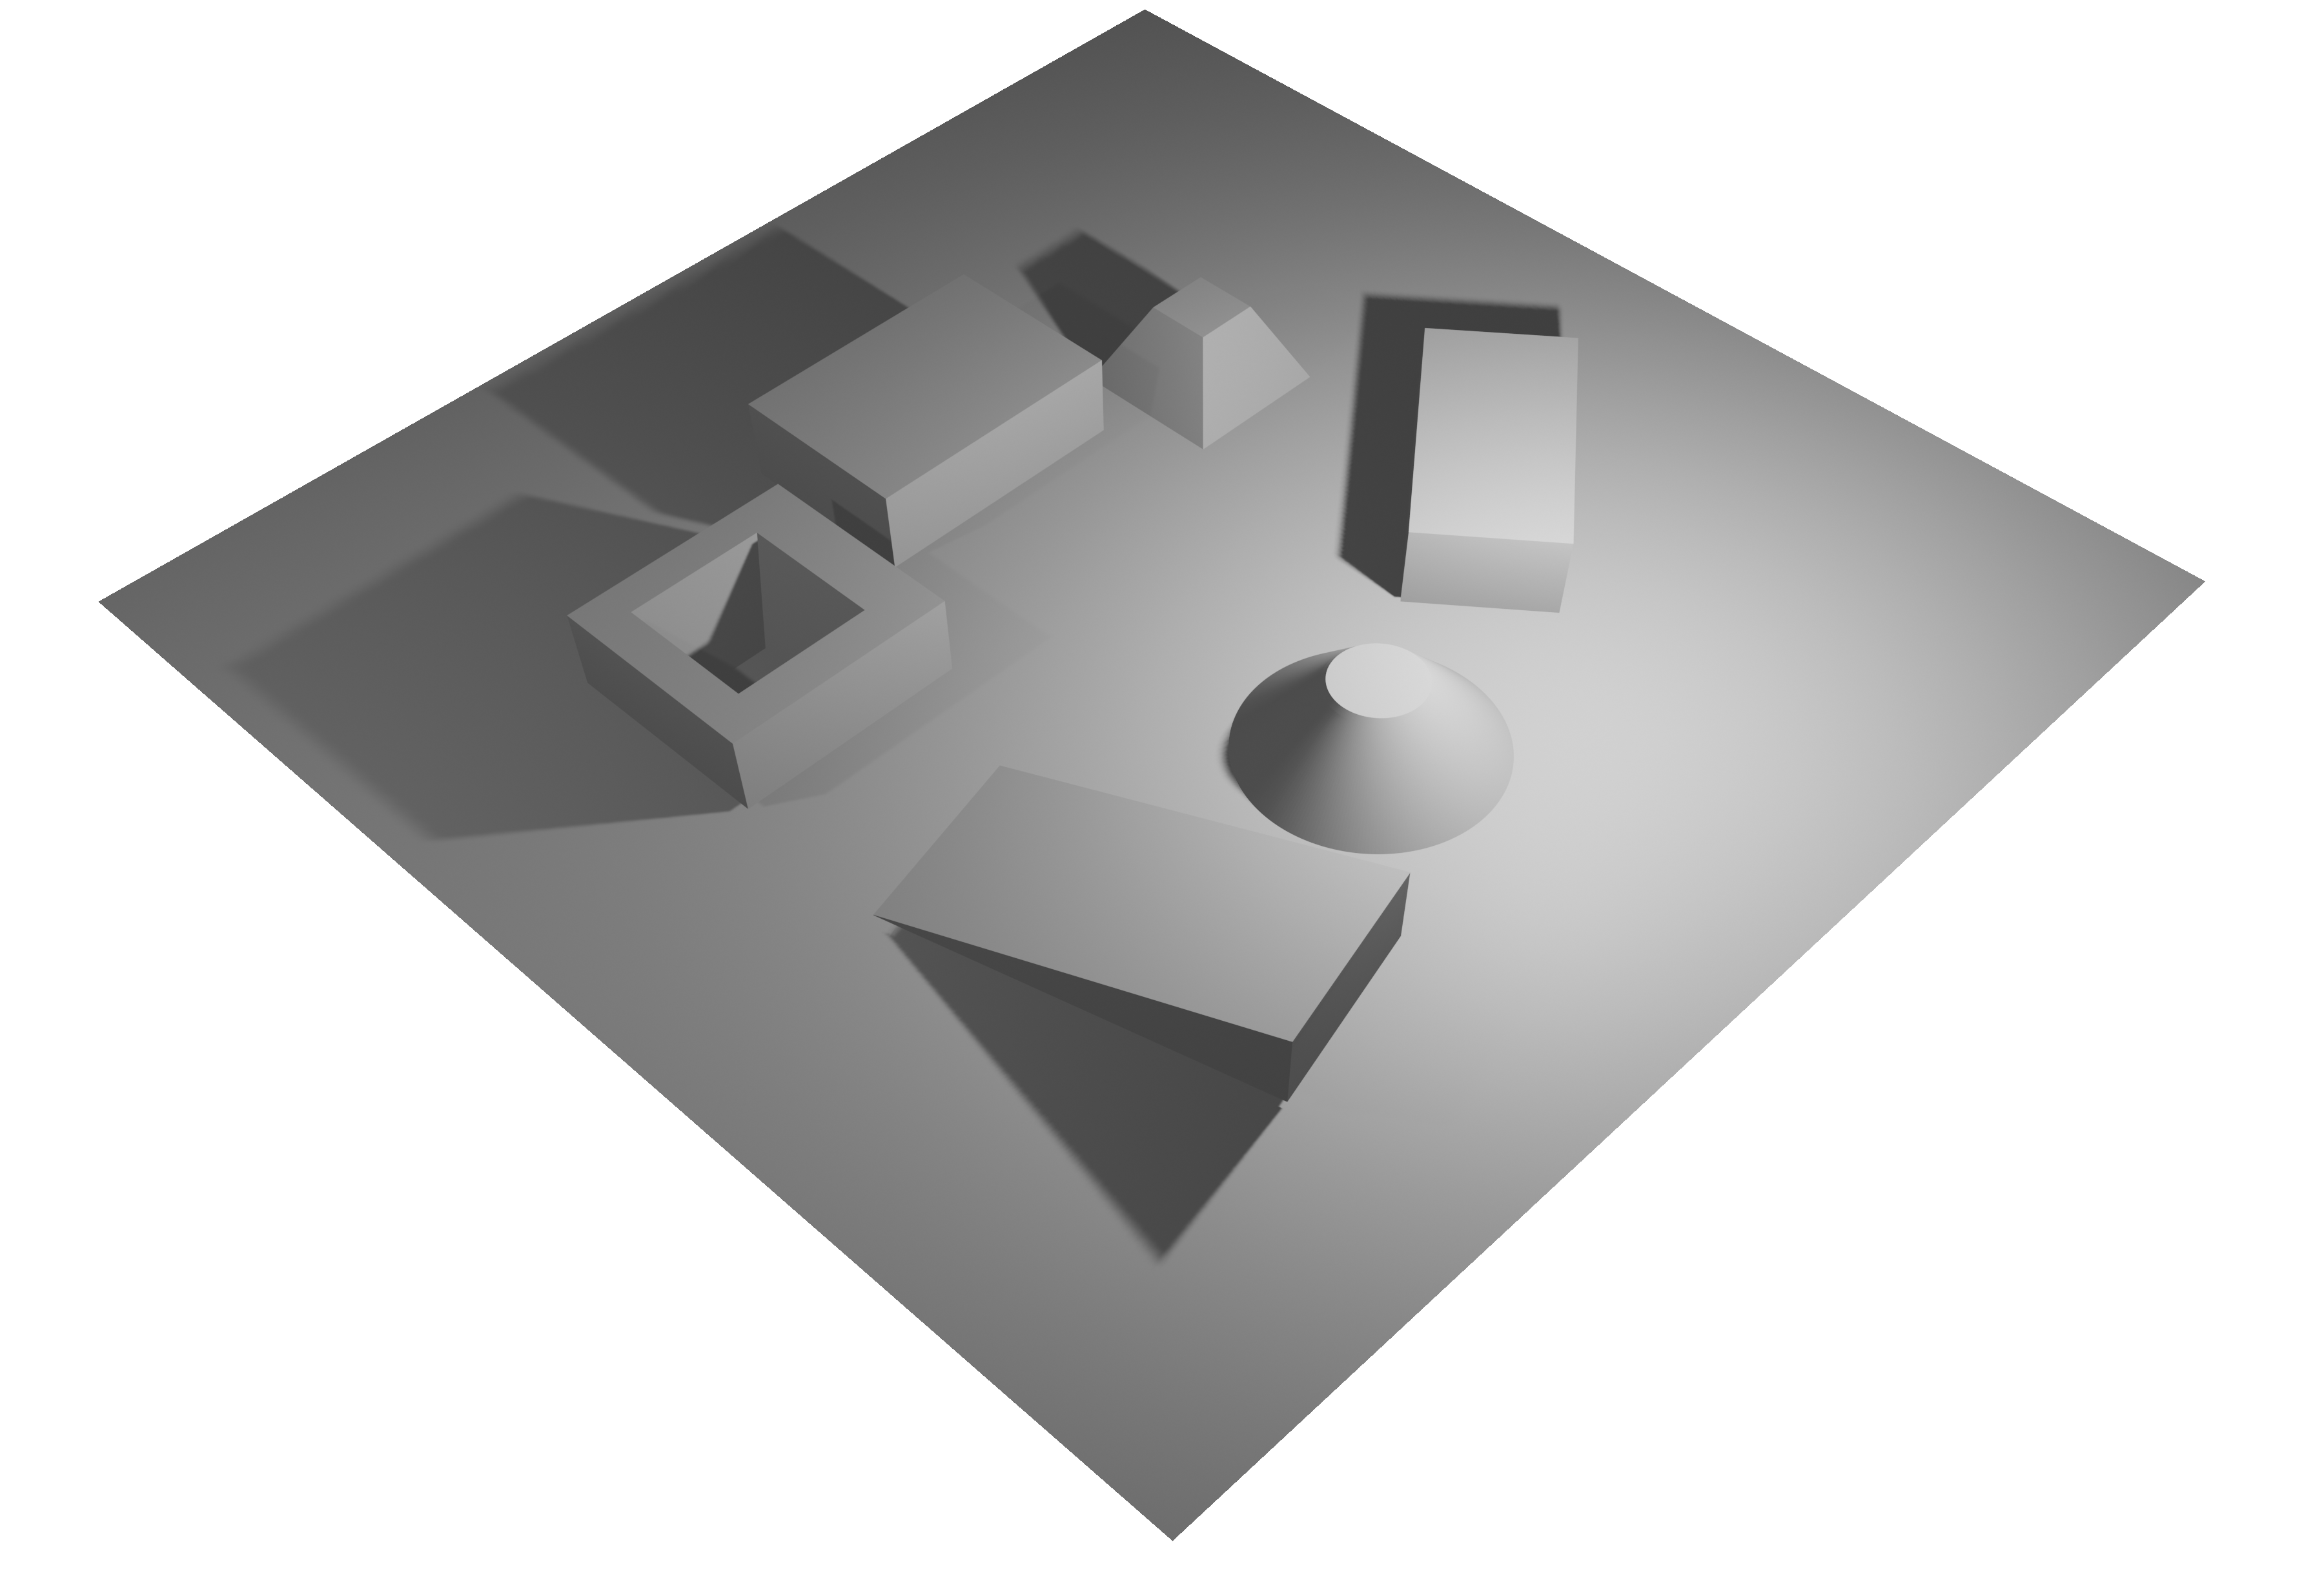
\includegraphics[height=.8\linewidth, left]{hmap3D.png}
            \caption{3D Terrain}
            \label{fig:sub_3d_terrain}
        \end{subfigure}%
        \begin{subfigure}{.5\textwidth}
            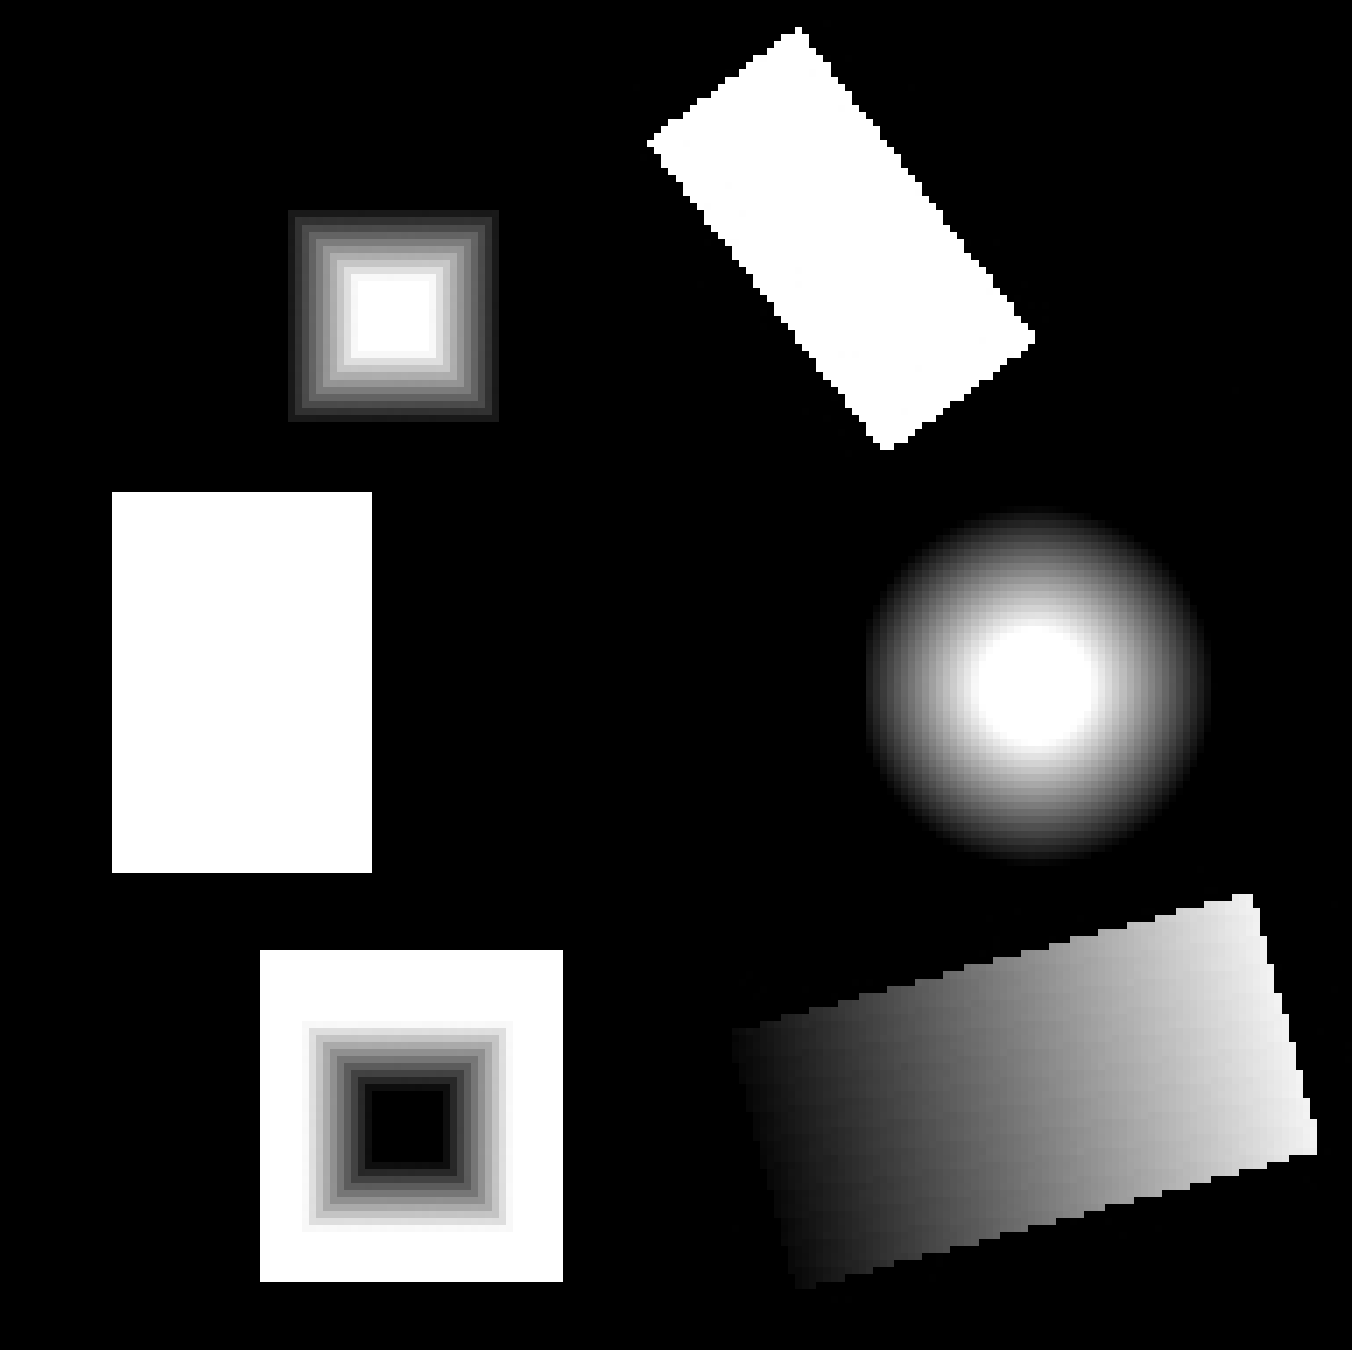
\includegraphics[height=.8\linewidth, right]{scoreTestHmap.png}
            \caption{Heightmap of 3D Terrain}
            \label{fig:sub_3d_terrain_hmap}
        \end{subfigure}
        \caption{3D Model of Terrain and its heightmap.}
        \label{fig:score_test_map}
    \end{figure}

    \noindent
    The heightmap in figure \ref{fig:sub_3d_terrain_hmap} is used to test the various walkability scores, first, in order to show individual results,
    the slope and edge proximity score is applied to the heightmap separately from each other, this is shown in figure \ref{fig:scores_seperate}. Next the combined score is
    shown in figure \ref{fig:full_score}, this is the score that is used to optimise foot end positions.
    \begin{figure}[h]
        \centering
        \begin{subfigure}{.45\textwidth}
            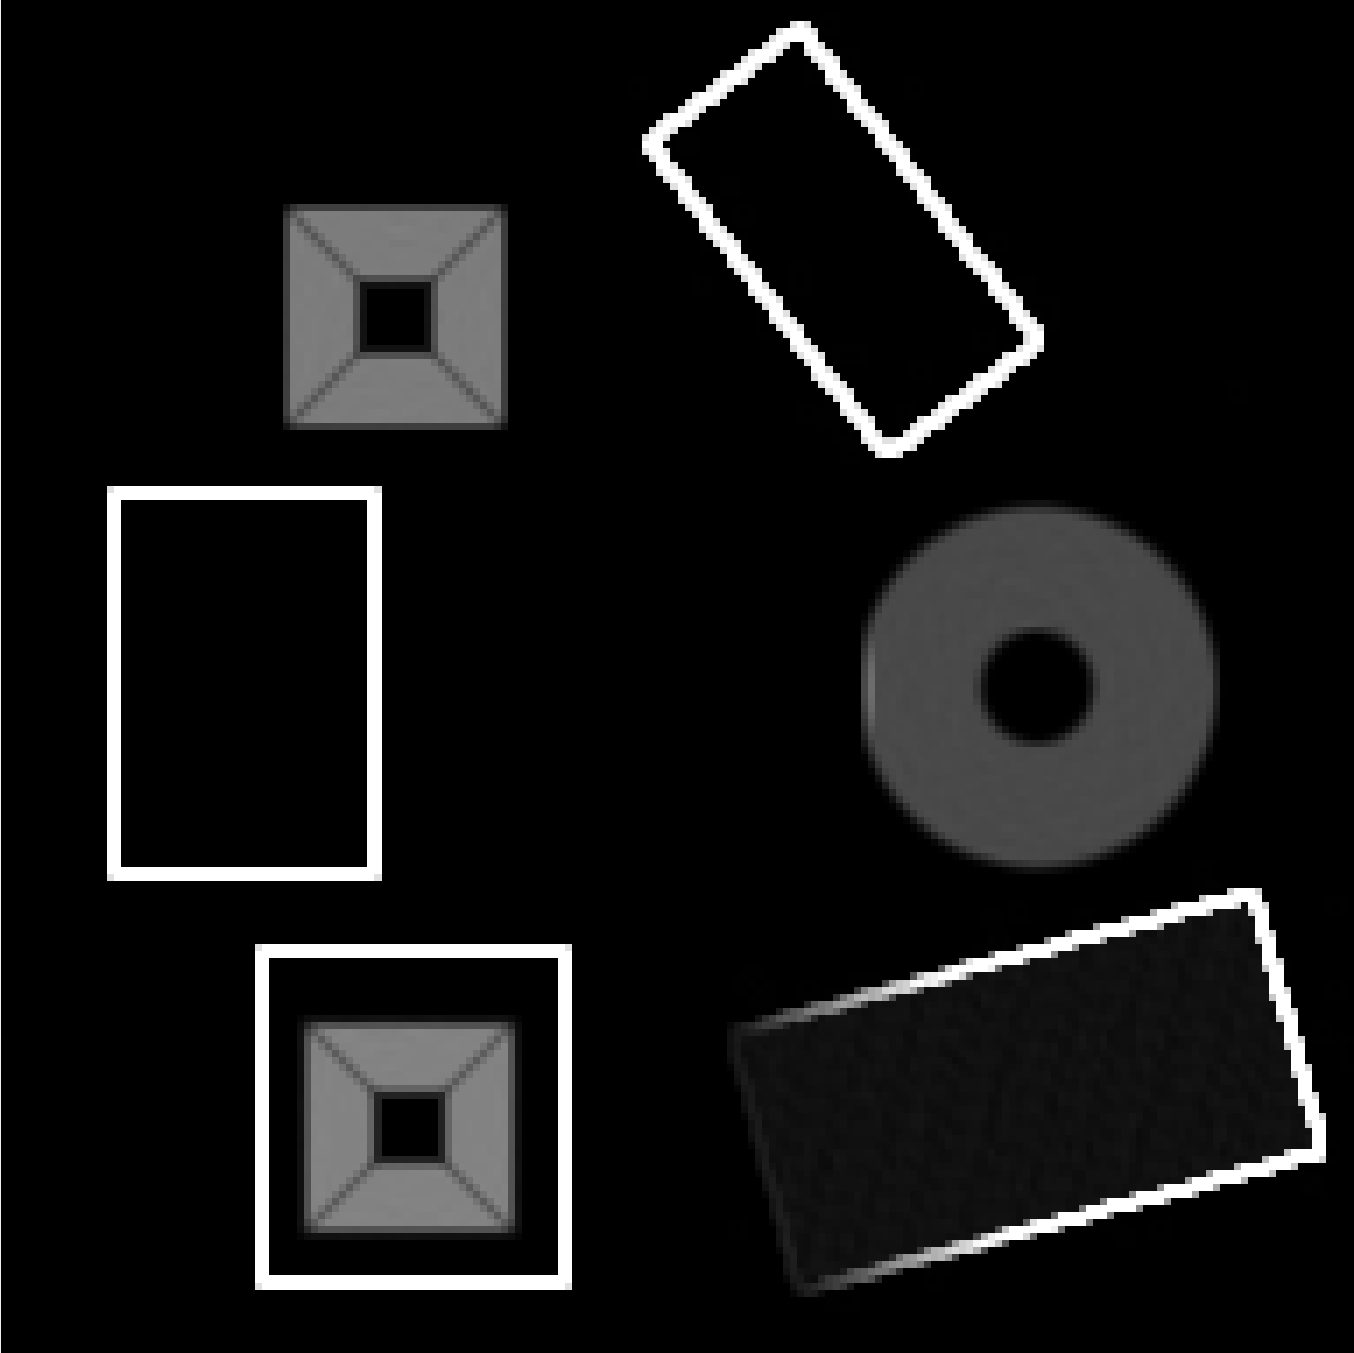
\includegraphics[height=.85\linewidth, left]{slopeScoreTest.png}
            \caption{Slope score test.}
            \label{fig:sub_slope_test}
        \end{subfigure}%
        \begin{subfigure}{.45\textwidth}
            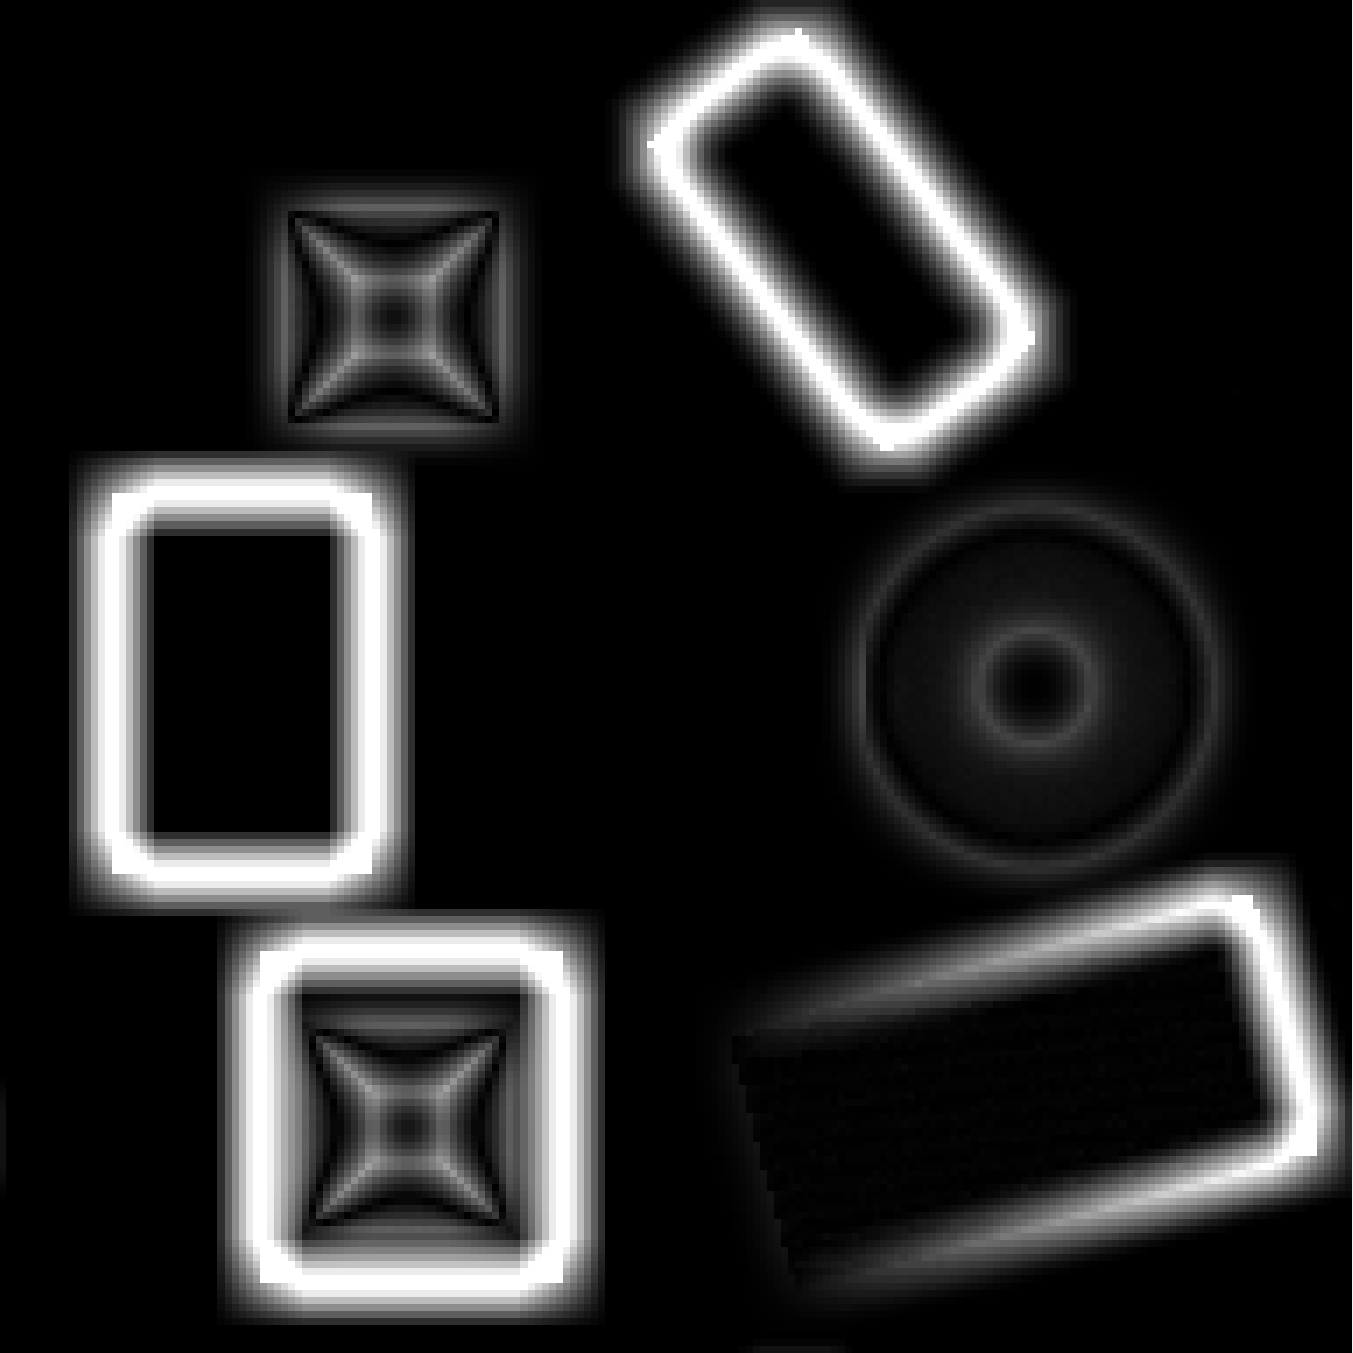
\includegraphics[height=.85\linewidth, right]{proxScoreTest.png}
            \caption{Edge proximity score test.}
            \label{fig:sub_prox_test}
        \end{subfigure}
        \caption{Slope score and edge proximity score tests.}
        \label{fig:scores_seperate}
    \end{figure}
    The slope score can be seen in figure \ref{fig:sub_slope_test}, from this it can be seen that the slope score successfully indicates sloped areas
    as less suitable foot end positions. It is also clear that vertical inclines are strongly discouraged, and while not the primary purpose of the slope
    score, this is expected and does not have a negative impact on scoring.

    Figure \ref{fig:sub_prox_test} shows that edge proximity score successfully discourages foot placement in areas with large height deviations,
    while allowing placement in areas with a locally similar slope, such as the ramp in the bottom-right. As can be seen from the larger, and more intense, discourage areas around the boxes in the
    top-right, bottom-right, left and bottom-left, it is clear that the magnitude of the height differential will increase the size and strength of the rejection area.
    Next, in figure \ref{fig:full_score} the combined slope and edge proximity scores can be seen. This is simply a weighted addition of the two scores.
    \begin{figure}[h]
        \centering
        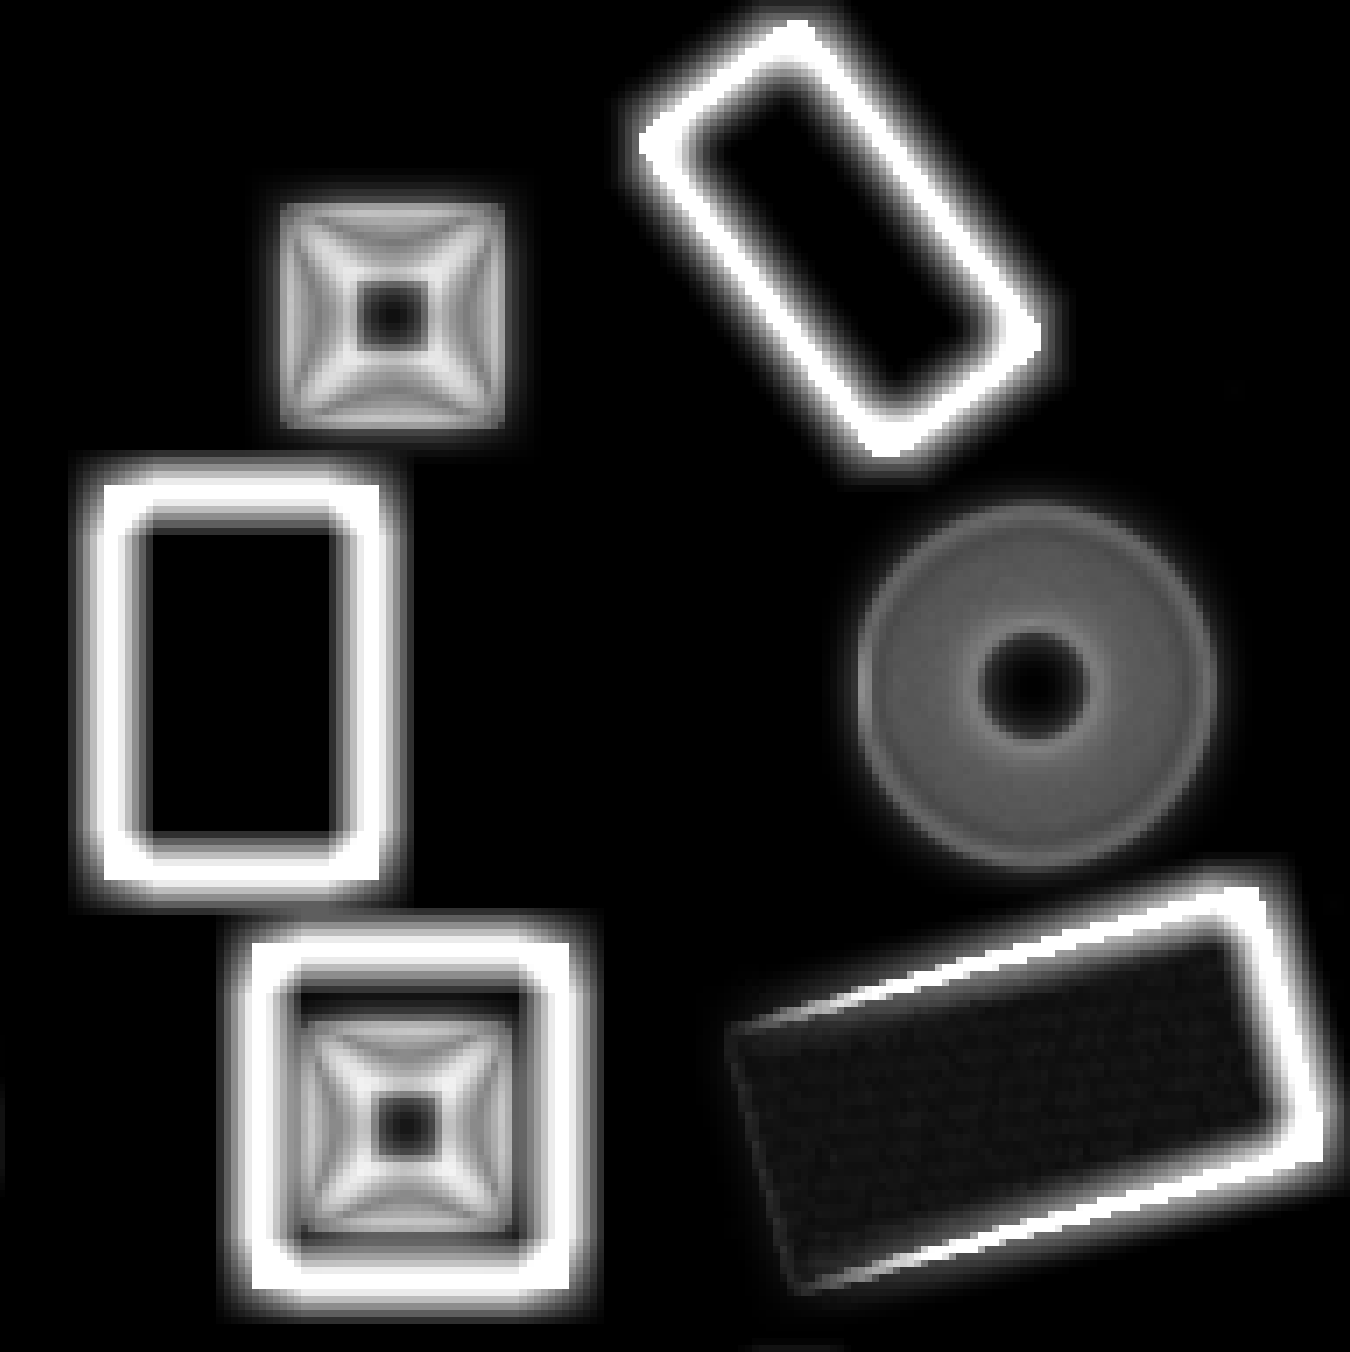
\includegraphics[width=.49\textwidth]{fullScore.png}
        \caption{Full walkability score.}
        \label{fig:full_score}
    \end{figure}

    Finally, the radial search algorithm described in section \ref{sec:radial_search} is used to optimise various nominal foot end positions.
    This is shown in figure \ref{fig:optimisation_test}.
    \begin{figure}[h]
        \centering
        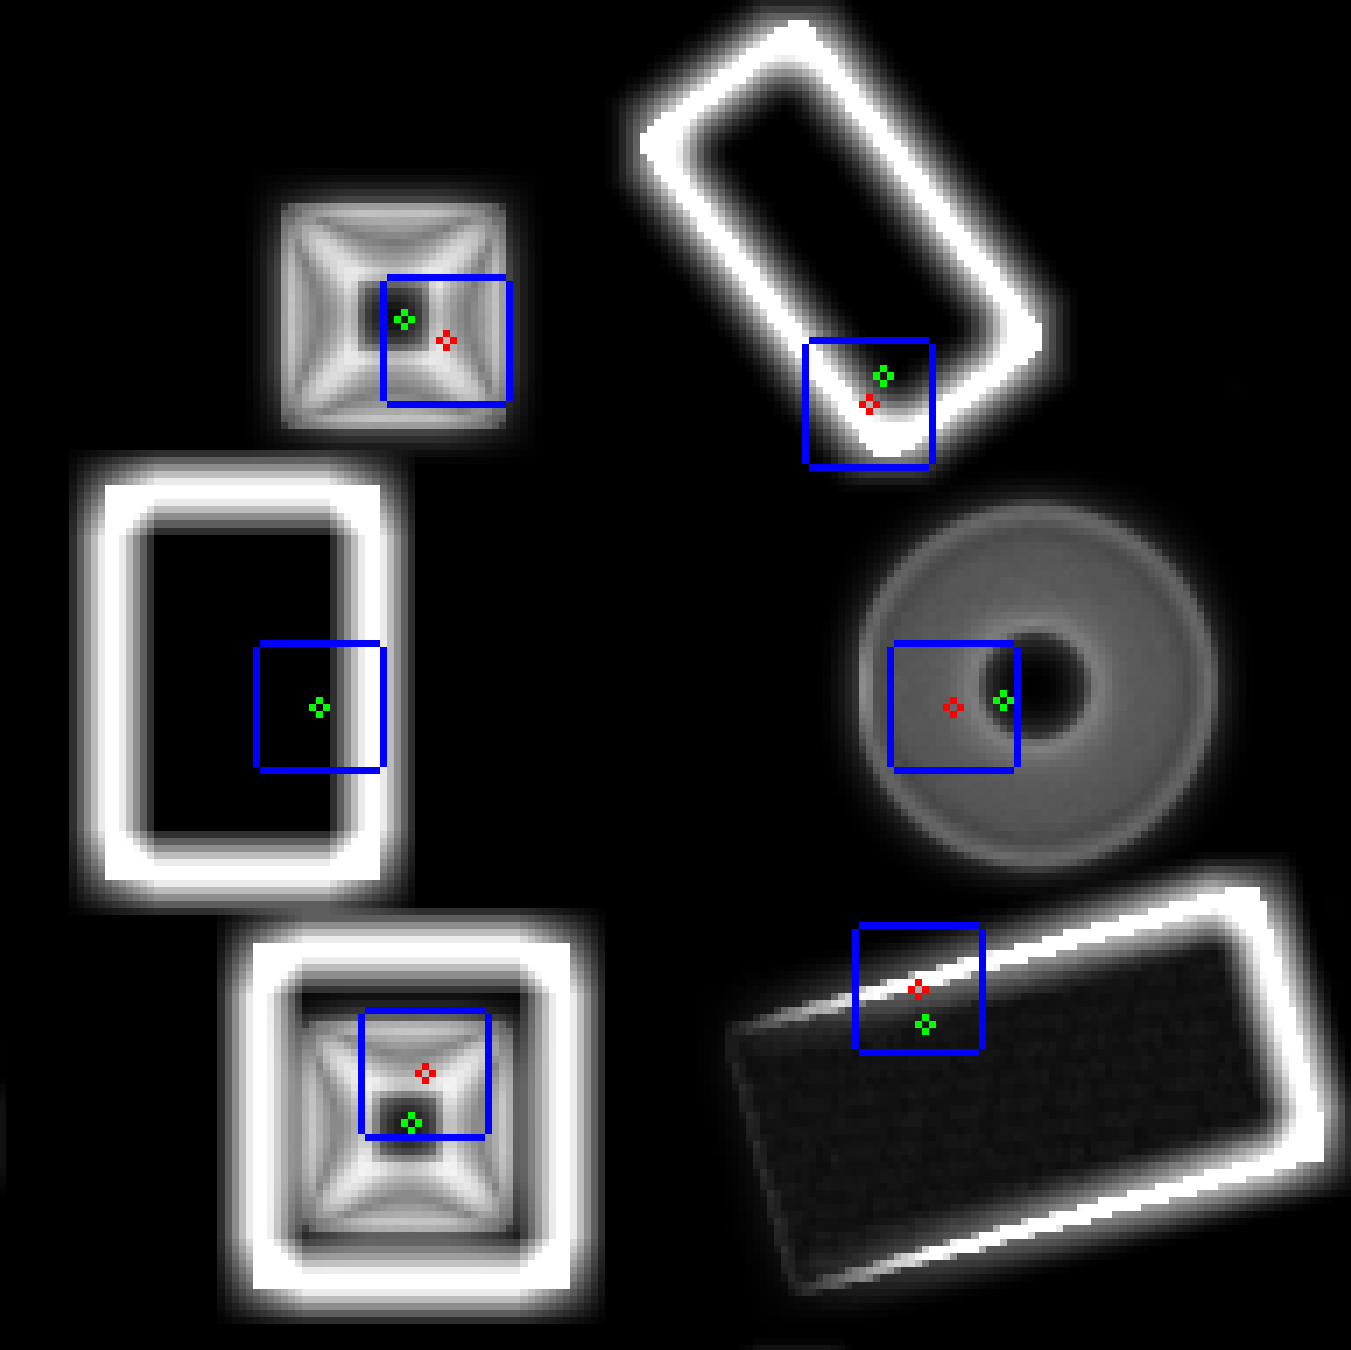
\includegraphics[width=.6\textwidth]{scoreTestFinal.png}
        \caption{Walkability score optimisation test.}
        \label{fig:optimisation_test}
    \end{figure}
    If the nominal foot position is in an acceptable position, the position will not be further optimised, this can be seen with the left most
    nominal position in figure \ref{fig:optimisation_test}. If however the nominal position is too close to an edge, such as with the top-right example, 
    the nominal position is optimised to the closest acceptable position. The optimised position does not need to have a perfect score, as can be seen in the bottom-right example, this example is similar to 
    the aforementioned top-right, but it adjusts onto the ram, which has a non-perfect, however acceptable, walkability score.
    Next the right most example shows how the nominal position is place on a piece of terrain that is too steep, this it is optimised onto the flat surface on top of the round pedestal. 
    
    Finally, the top-left and bottom-left examples show the case of a nominal position placed on a sloped pillar and a sloped hole respectively.
    In both cases the nominal position is optimised to the flat surface at the to of the pillar and at the bottom of the hole.
    
    The flat surfaces on the pillar an in the hole are large enough to not be rejected by the edge proximity score, however, if the inclines sere steeper or the flat surface smaller it is possible that these nominal positions would be
    unsolvable, as there is no appropriate foot end placement inside the search radius. In this case the robot would need to make a course adjustment.

\newpage
\section{Walking}
    The final walking tests are comprised of three different terrains, a simple flat plane as a baseline, then a staircase to demonstrate simple foot and body height adjustment and
    finally a uneven organic like surface.
    
    When presenting testing data, a snapshot of the 3D simulation environment will be shown, with the body and foot paths traced. Additionally key data points
    are also graphed, however only the height of a single foot will be graphed, this is to maintain clarity.

    \subsection{Flat Plane}
    The flat plane test aims to quantify nominal body height oscillations and to provide a baseline to compare subsequent test to.
    Figure \ref{fig:plane_test} and \ref{fig:plane_test_data} shows the test results of walking over a simple flat plane, as expected the the step sizes and arcs are uniform with no optimisation necessary.
    \begin{figure}[h]
        \centering
        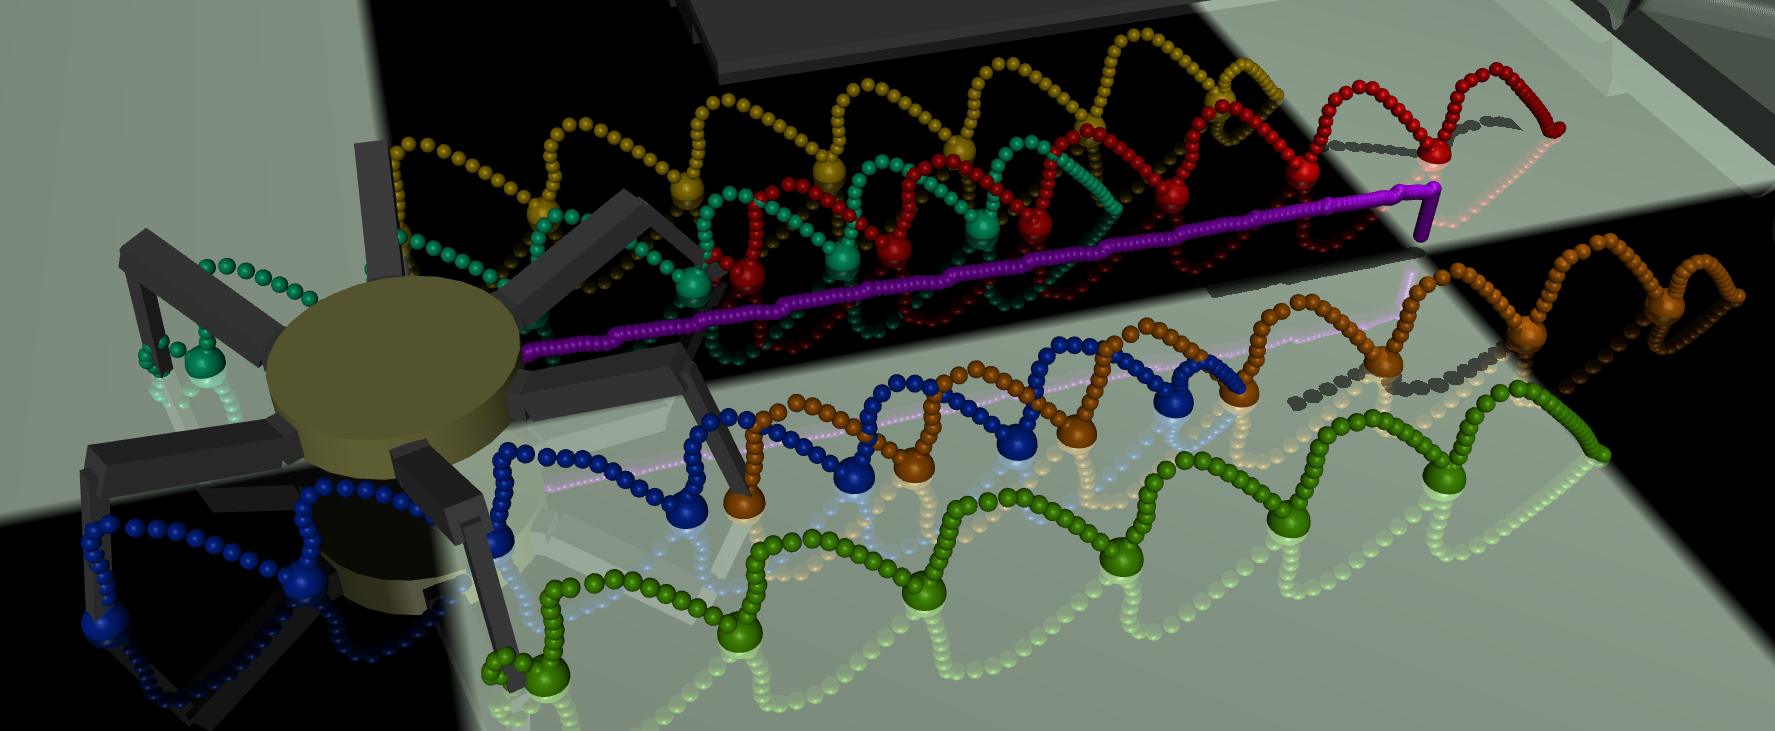
\includegraphics[width=.8\textwidth]{WalkTestPlane.png}
        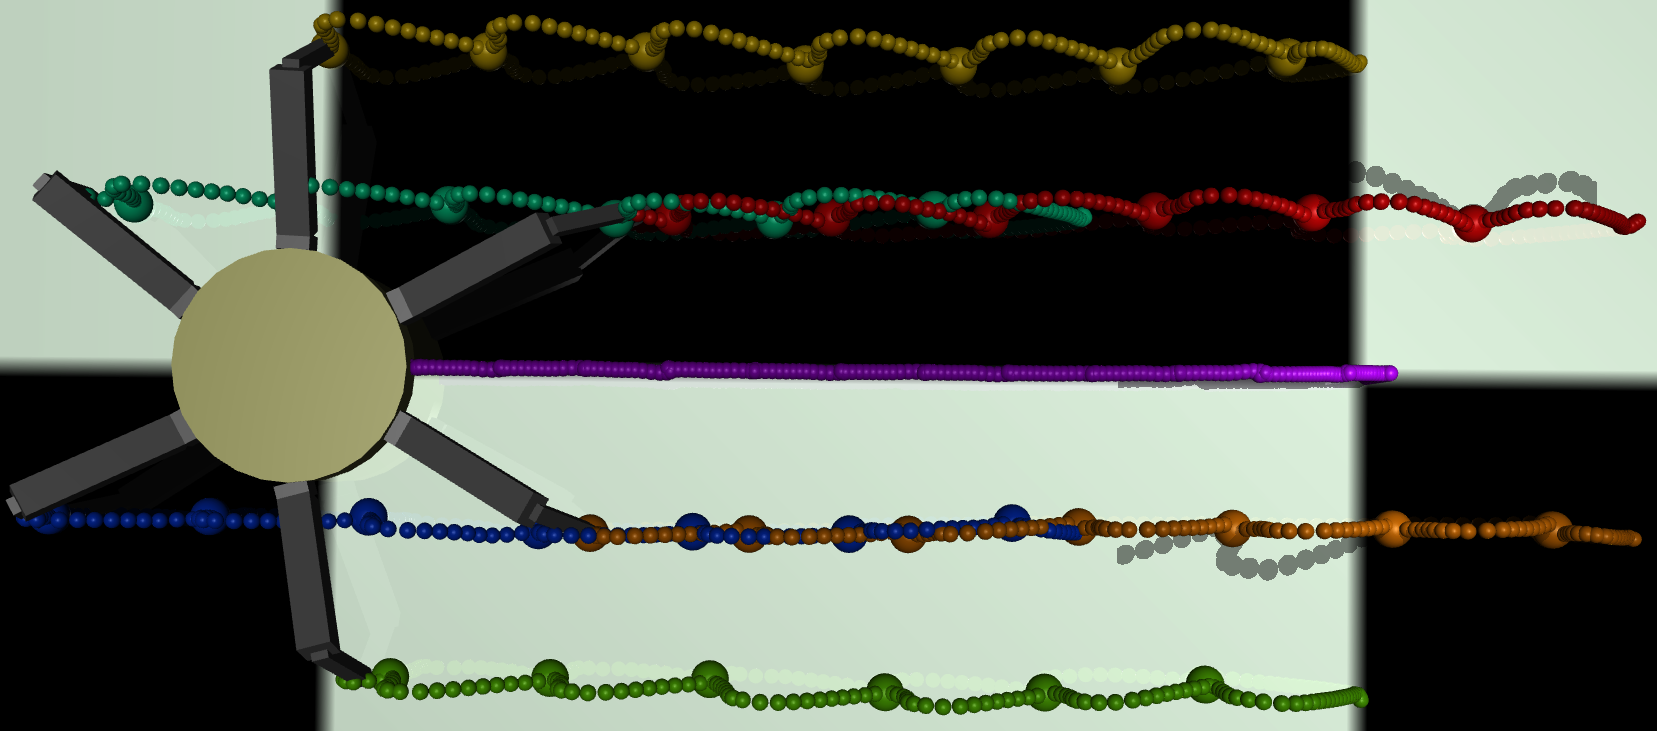
\includegraphics[width=.8\textwidth]{WalkTestPlaneTop.png}
        \caption{Flat plane walk test}
        \label{fig:plane_test}
    \end{figure}
    \begin{figure}[h]
        \centering
        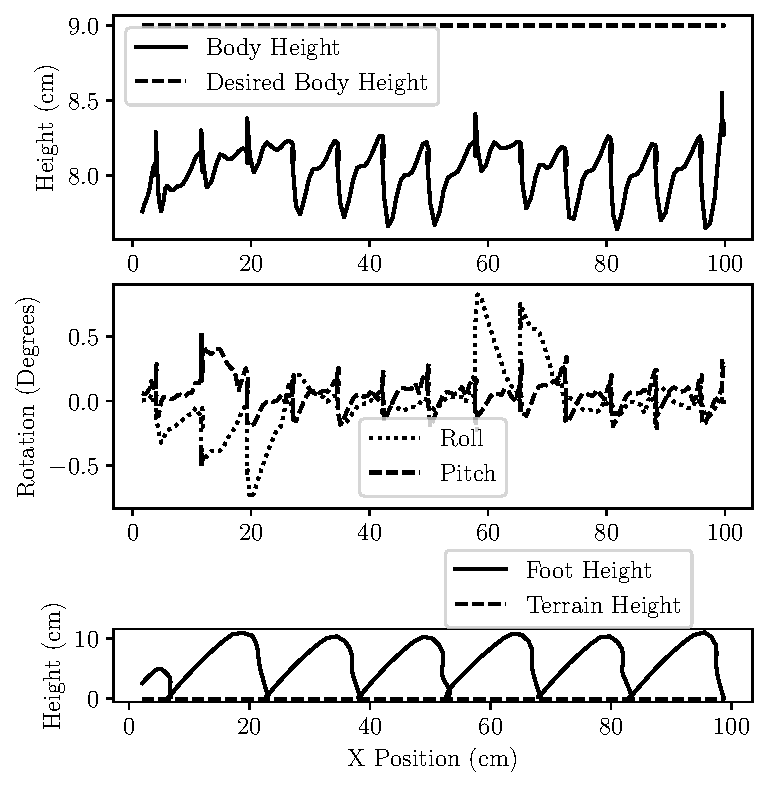
\includegraphics{data_plane.pdf}
        \caption{Body height (top). Body tilt (center). Position of one foot (bottom)}
        \label{fig:plane_test_data}
    \end{figure}
    
    \noindent
    From figure \ref{fig:plane_test_data} it can be seen that there is a constant error of about 1cm in the body height of the robot, this can be easily solved by adding a constant offset or adding integral 
    control to the leg servos. It is also clear that as the robot walks there are some oscillations in the body height, this is to be expected and the oscillations are lower than the \(10\%\) desired body height specification.
        
    Next it can be seen that the tilt of the body, in both roll and pitch, tends to stay below \(0.5^\circ\), which is well within specifications. It is also possible to further improve
    the tilt error by incorporating accelerometer based feedback control to the feet heights. Finally, the height of one of the legs are shown, from this it is clear that the robot takes
    uniform, stable steps.

    \newpage
    \subsection{Staircase}
    The staircase test demonstrates the ability of the robot to adjust the height of its feet in order to maintain a level body,
    additionally the ability of the robot to automatically adjust its height relative to the floor is also demonstrated. A 3D image
    of this test can be seen in figure \ref{fig:stairs_test} and the data plots in figure \ref{fig:stairs_test_data}.
    \begin{figure}[h]
        \centering
        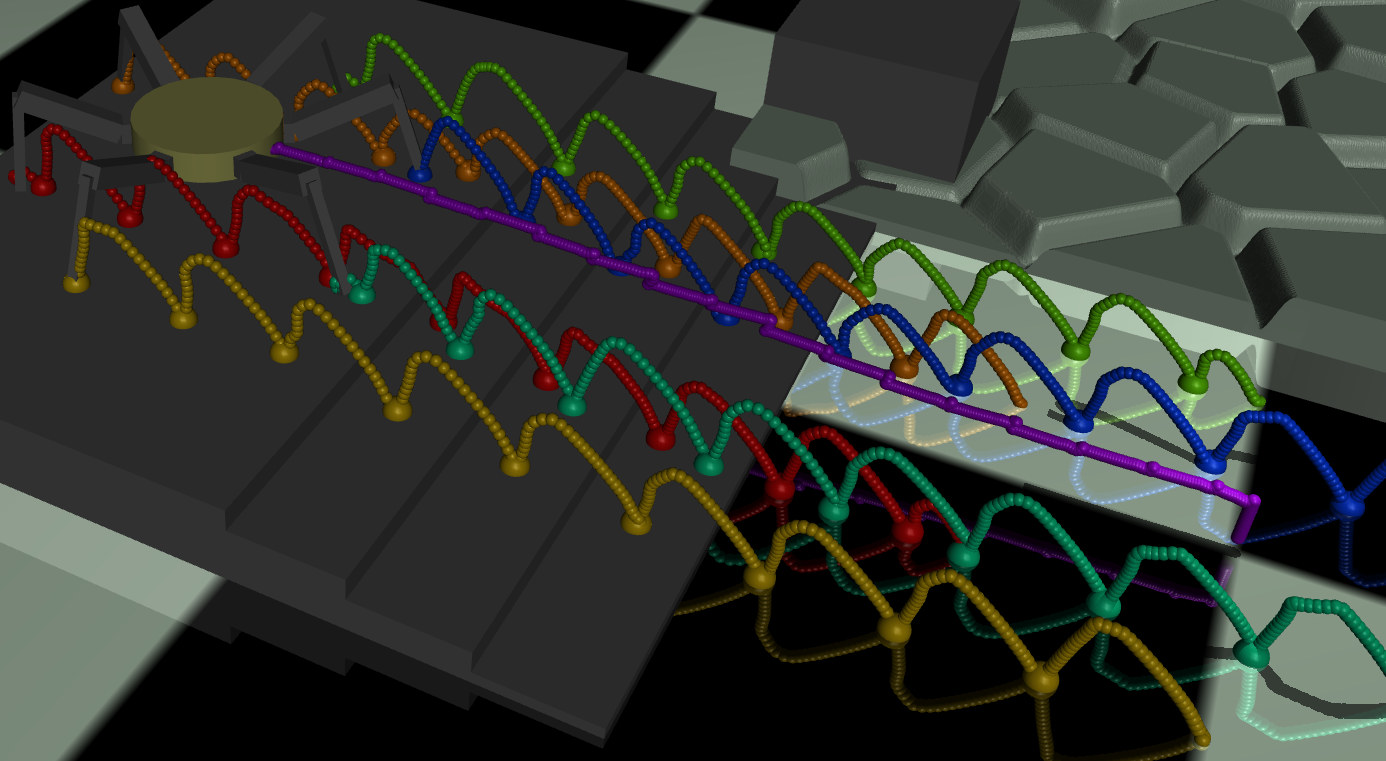
\includegraphics[width=.8\textwidth]{WalkTestStairts.png}
        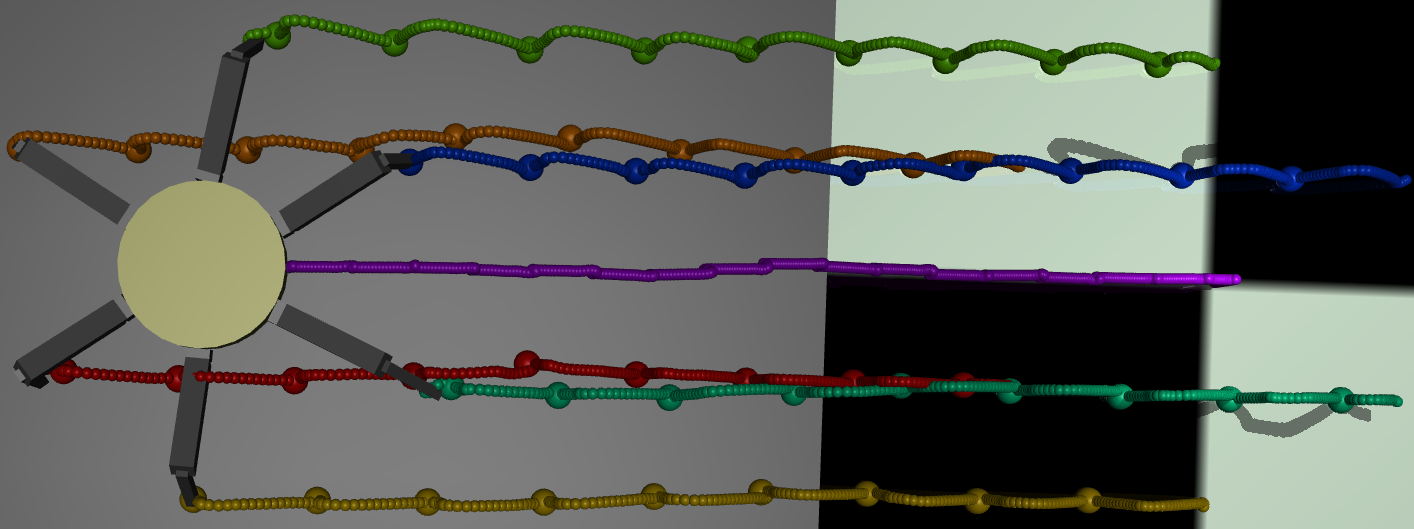
\includegraphics[width=.8\textwidth]{WalkTestStairtsTop.png}
        \caption{Stairs walk test}
        \label{fig:stairs_test}
    \end{figure}
    \begin{figure}[h]
        \centering
        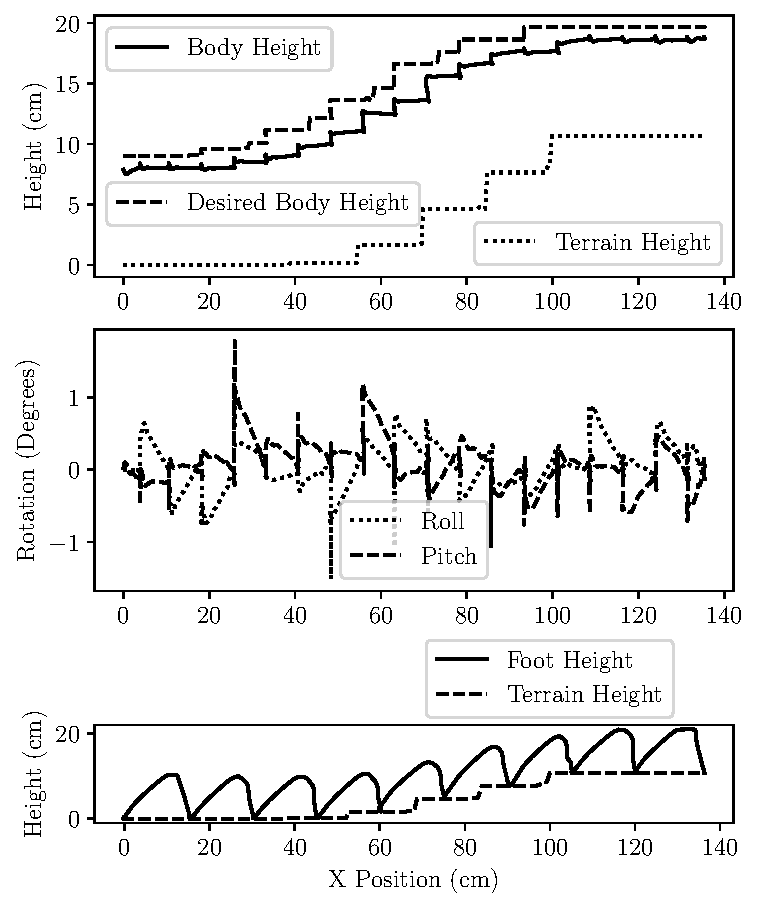
\includegraphics{data_stairs.pdf}
        \caption{Body height (top). Body tilt (center). Position of one foot (bottom)}
        \label{fig:stairs_test_data}
    \end{figure}

    Similarly to the flat plane test, as expected, the constant body height error is still present.
    However, from this test it can be seen in figure \ref{fig:stairs_test_data} that the robot does increase its height to maintain a constant
    height above the terrain. It is clear that the body height is not increased in the four discrete steps as the stairs do, rather the
    body height is increased more smoothly using many smaller steps. This is thanks to the system described in section \ref{sec:height_adjust}.

    Body tilt, while more prominent than in the flat plane test, is still quite low as it largely stays below \(1.0^\circ\), with intermittent jumps approaching \(2.0^\circ\).
    This is still within the specifications, and as previously stated could easily be improved by incorporating accelerometer based feedback control on the foot height.

    Finally, the foot height plot clearly shows how one of the feet of the robot adjusts its height and step arc based on the terrain. Otherwise the foot arc looks very similar to that of the
    flat plane test, which is optimal.
    
    \newpage
    \subsection{Organic}
    The organic test aims to show how the robot can place feet on an appropriate spot on the terrain, while maintaining level and a certain height. Figure \ref{fig:org_test} shows the
    3D view of the test.
    \captionsetup[figure]{oneside,margin={0.9cm,0cm}}
    \begin{figure}[h]
        \centering
        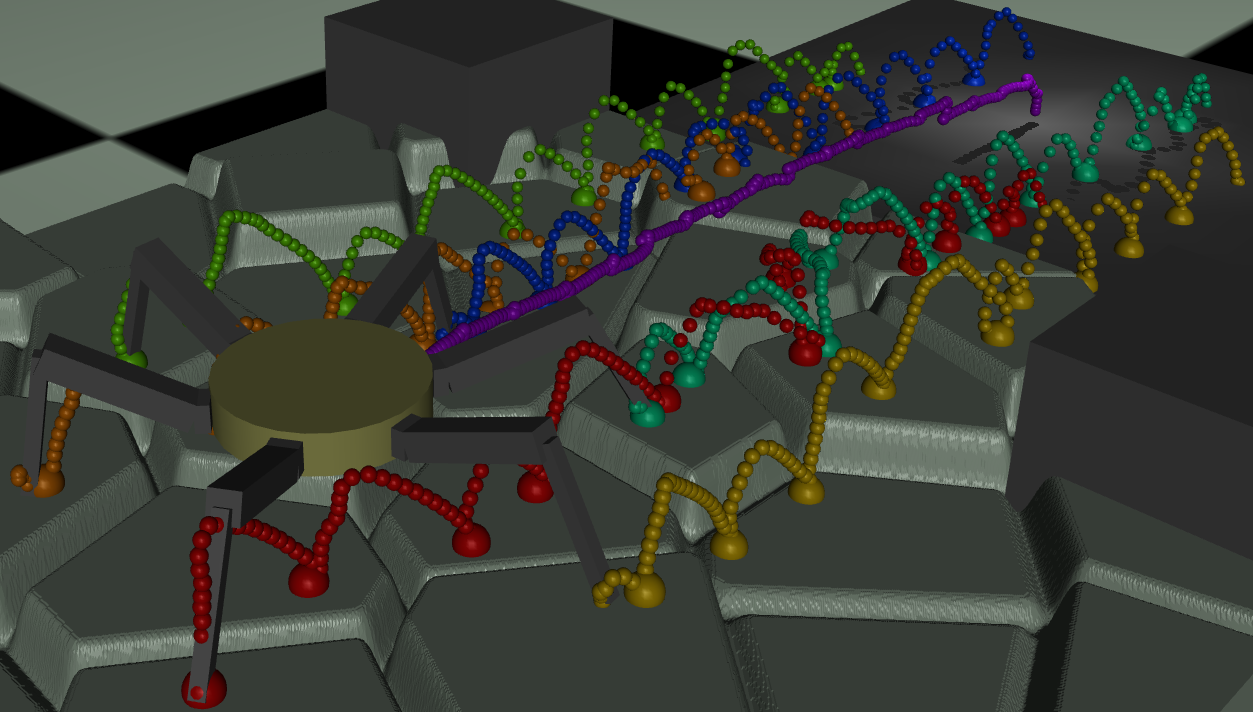
\includegraphics[width=.8\textwidth]{WalkTestOrg.png}
        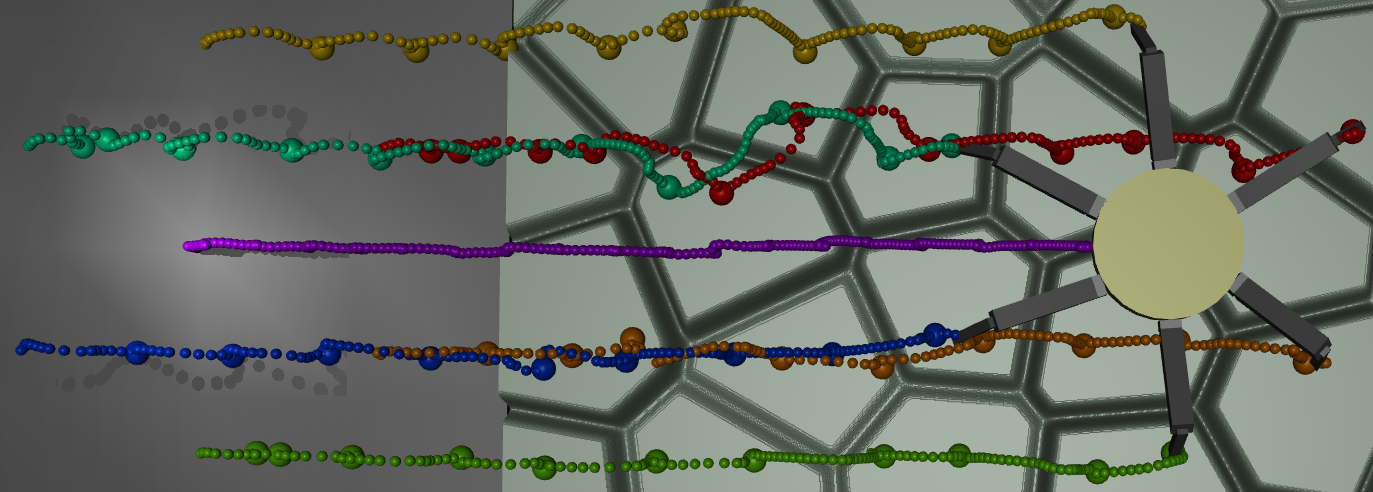
\includegraphics[width=.8\textwidth]{WalkTestOrgTop.png}
        \caption{Organic walk test.}
        \label{fig:org_test}
    \end{figure}
    \begin{figure}[h]
        \centering
        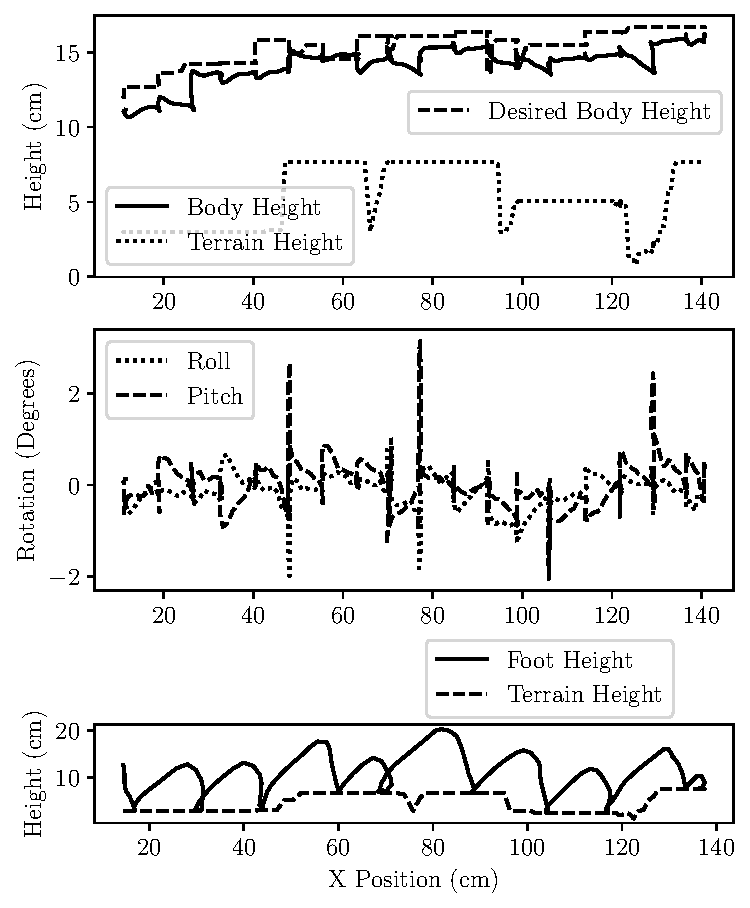
\includegraphics{data_org.pdf}
        \caption{Body height (top). Body tilt (center). Position of one foot (bottom)}
        \label{fig:org_test_data}
    \end{figure}

    From figure \ref{fig:org_test_data} it can be seen that the body height error seen in the flat plane test
    is still present and more severe. But the body does stay within a reasonable margin from the desired height.

    For most part the body tilt is similar to that of the stairs test, however more frequent and more sever spikes are present.
    This is due, in part, to the more erratic mismatch between the body height and the requested body heigh. The horizontal adjustments made to 
    the foot end positions cause the swinging feet to end their steps at different times, this is the primary cause of the tilt spikes, as when one
    foot is placed on the floor before the other two, the robot is tilted slightly. This, however, would not occur if there was no, or little, 
    error in the body height.

    Finally, when looking at the foot position plot in figure \ref{fig:org_test_data}, please note that the plot is a projection into the X-Z plane, and thus any
    adjustment made in the Y-axis is not shown, the foot shown has been chosen to include minimum Y-axis variation. 
    Thus, please also see the 3D view in figure \ref{fig:org_test}. From these two figures it is clear that the foot end positions are, in addition to height,
    adjusted in the horizontal plane, the step arcs are appropriately adjusted and remain relatively smooth, similar to the flat plane test.
